\chapter{Experiment 0: Fundamentals of Arduino Interfacing}

%%%%%%%%%%%%%%%%%%%%%%%%%%%%%%%%%%%%%%%%%%%%%%%%%%%%%%%%%%%%%%%%%%%%%%%
\section{LED Flash System}

\subsection{Problem Statement}

The objective of this experiment is to interface an LED with an Arduino Uno and make it blink continuously at a fixed interval.

This experiment helps to understand:

\begin{itemize}
    \item Digital output pins of Arduino
    \item Basic Arduino programming structure
    \item Use of functions in Arduino
    \item Timing control using \texttt{delay()}
\end{itemize}

%%%%%%%%%%%%%%%%%%%%%%%%%%%%%%%%%%%%%%%%%%%%%%%%%%%%%%%%%%%%%%%%%%%%%%%

\subsection {Components Used \& Pin Connections}


\begin{table}[H]
\centering

\begin{minipage}{0.48\textwidth}
\centering
\caption{LED Flash Components}
\label{tab:ledflash_components}
\begin{tabular}{|l|c|}
\hline
\textbf{Component} & \textbf{Quantity} \\
\hline
Arduino UNO & 1 \\
LED & 1 \\
100$\Omega$ Resistor & 1 \\
Breadboard & 1 \\
Jumper Wires & Required \\
\hline
\end{tabular}
\end{minipage}
\hfill
\begin{minipage}{0.48\textwidth}
\centering
\caption{LED Flash Pin Connections}
\label{tab:ledflash_pins}
\begin{tabular}{|l|l|}
\hline
\textbf{Device} & \textbf{Arduino Pin} \\
\hline
LED Positive Terminal & D12 \\
LED Negative Terminal & GND \\
\hline
\end{tabular}
\end{minipage}

\end{table}

%%%%%%%%%%%%%%%%%%%%%%%%%%%%%%%%%%%%%%%%%%%%%%%%%%%%%%%%%%%%%%%%%%%%%%%

\subsection{Software Used}

\begin{itemize}
    \item Arduino IDE
    \item SimulIDE
\end{itemize}

%%%%%%%%%%%%%%%%%%%%%%%%%%%%%%%%%%%%%%%%%%%%%%%%%%%%%%%%%%%%%%%%%%%%%%%

\subsection{Circuit Diagram}

\begin{figure}[H]
\centering

\includegraphics[width=0.55\textwidth]{Exp-0/led_flash/led_flash.png}
\caption{Circuit Diagram of LED Flash System}
\label{fig:led_flash}
\end{figure}

%%%%%%%%%%%%%%%%%%%%%%%%%%%%%%%%%%%%%%%%%%%%%%%%%%%%%%%%%%%%%%%%%%%%%%%

\subsection{Source Code}

The complete Arduino source code for this experiment is available in the project repository.

\href{https://github.com/YOUR_USERNAME/YOUR_REPOSITORY/blob/main/Exp-0/led_flash/led_flash.ino}
{\textbf{Click here to view the Arduino Source Code}}

%%%%%%%%%%%%%%%%%%%%%%%%%%%%%%%%%%%%%%%%%%%%%%%%%%%%%%%%%%%%%%%%%%%%%%%

\subsection{Working Principle}

\begin{enumerate}
    \item The LED is connected to digital pin D12 of Arduino UNO.

    \item In the \texttt{setup()} function, pin D12 is configured as an output pin using \texttt{pinMode()}.

    \item The \texttt{loop()} function continuously calls the \texttt{toggle\_led()} function.

    \item Inside the \texttt{toggle\_led()} function:
    \begin{itemize}
        \item The LED turns ON using \texttt{digitalWrite(HIGH)}
        \item Arduino waits for 1 second using \texttt{delay(1000)}
        \item The LED turns OFF using \texttt{digitalWrite(LOW)}
        \item Arduino again waits for 1 second
    \end{itemize}

    \item This process repeats continuously, causing the LED to blink repeatedly.
\end{enumerate}

%%%%%%%%%%%%%%%%%%%%%%%%%%%%%%%%%%%%%%%%%%%%%%%%%%%%%%%%%%%%%%%%%%%%%%%

\subsection{What I Learned}

\begin{itemize}
    \item Arduino UNO digital pins give approximately 5V output.
    \item Recommended current per digital pin is 20mA.
    \item Maximum current per digital pin is 40mA.
    \item Typical LED operating current is around 10mA to 20mA.
    \item LEDs should be connected using a current-limiting resistor.
    \item Basic LED interfacing with Arduino UNO.
\end{itemize}

%%%%%%%%%%%%%%%%%%%%%%%%%%%%%%%%%%%%%%%%%%%%%%%%%%%%%%%%%%%%%%%%%%%%%%%

\subsection{Conclusion}

The LED Blinking System using Arduino UNO was successfully implemented and tested.

The LED blinked continuously with a delay of 1 second ON and 1 second OFF. This experiment helped in understanding basic Arduino programming, digital output control, and hardware interfacing.

%%%%%%%%%%%%%%%%%%%%%%%%%%%%%%%%%%%%%%%%%%%%%%%%%%%%%%%%%%%%%%%%%%%%%%%


\subsection{References}

\begin{enumerate}
    \item Arduino Official Website

    \url{https://www.arduino.cc/}

    \item Arduino UNO Documentation

    \url{https://docs.arduino.cc/hardware/uno-rev3/}

    \item Arduino Tutorials

    \url{https://www.arduino.cc/en/Tutorial/HomePage}

    \item Arduino IDE Documentation

    \url{https://docs.arduino.cc/software/ide/}

    \item SimulIDE

    \url{https://simulide.com/}

    
\end{enumerate}

\clearpage

\textit{Experiment 0 -- Go Further 1}
%%%%%%%%%%%%%%%%%%%%%%%%%%%%%%%%%%%%%%%%%%%%%%%%%%%%%%%%%%%%%%%%%%%%%%%
\section{7-Segment Display Interfacing}


%%%%%%%%%%%%%%%%%%%%%%%%%%%%%%%%%%%%%%%%%%%%%%%%%%%%%%%%%%%%%%%%%%%%%%%
\subsection{Problem Statement}

The objective of this project is to interface a common-cathode 7-segment display with an Arduino Uno and display numbers sequentially.

This experiment helps in understanding:

\begin{itemize}
    \item 7-segment display interfacing
    \item Digital output control
    \item Number display logic
    \item Multi-pin control using Arduino
\end{itemize}

%%%%%%%%%%%%%%%%%%%%%%%%%%%%%%%%%%%%%%%%%%%%%%%%%%%%%%%%%%%%%%%%%%%%%%%

\subsection {Components Used \& Pin Connections}
\begin{table}[H]
\centering

\begin{minipage}{0.48\textwidth}
\centering
\caption{7-Segment Components}
\label{tab:7segment_components}

\begin{tabular}{|p{5cm}|c|}
\hline
\textbf{Component} & \textbf{Quantity} \\
\hline
Arduino UNO & 1 \\
7-Segment Display(Common Cathode) & 1 \\
220$\Omega$ Resistors & 7 \\
Jumper Wires & Required \\
Breadboard & 1 \\
\hline
\end{tabular}

\end{minipage}
\hfill
\begin{minipage}{0.48\textwidth}
\centering
\caption{7-Segment Pin Connections}
\label{tab:7segment_pins}

\begin{tabular}{|c|c|}
\hline
\textbf{7-Segment Pin} & \textbf{Arduino Pin} \\
\hline
a & D2 \\
b & D3 \\
c & D4 \\
d & D5 \\
e & D6 \\
f & D7 \\
g & D8 \\
\hline
\end{tabular}

\end{minipage}

\end{table}

%%%%%%%%%%%%%%%%%%%%%%%%%%%%%%%%%%%%%%%%%%%%%%%%%%%%%%%%%%%%%%%%%%%%%%%

\subsection{Software Used}

\begin{itemize}
    \item Arduino IDE
    \item SimulIDE
\end{itemize}

%%%%%%%%%%%%%%%%%%%%%%%%%%%%%%%%%%%%%%%%%%%%%%%%%%%%%%%%%%%%%%%%%%%%%%%

\subsection{Circuit Diagram}

\begin{figure}[H]
\centering

\begin{minipage}{0.48\textwidth}
    \centering
    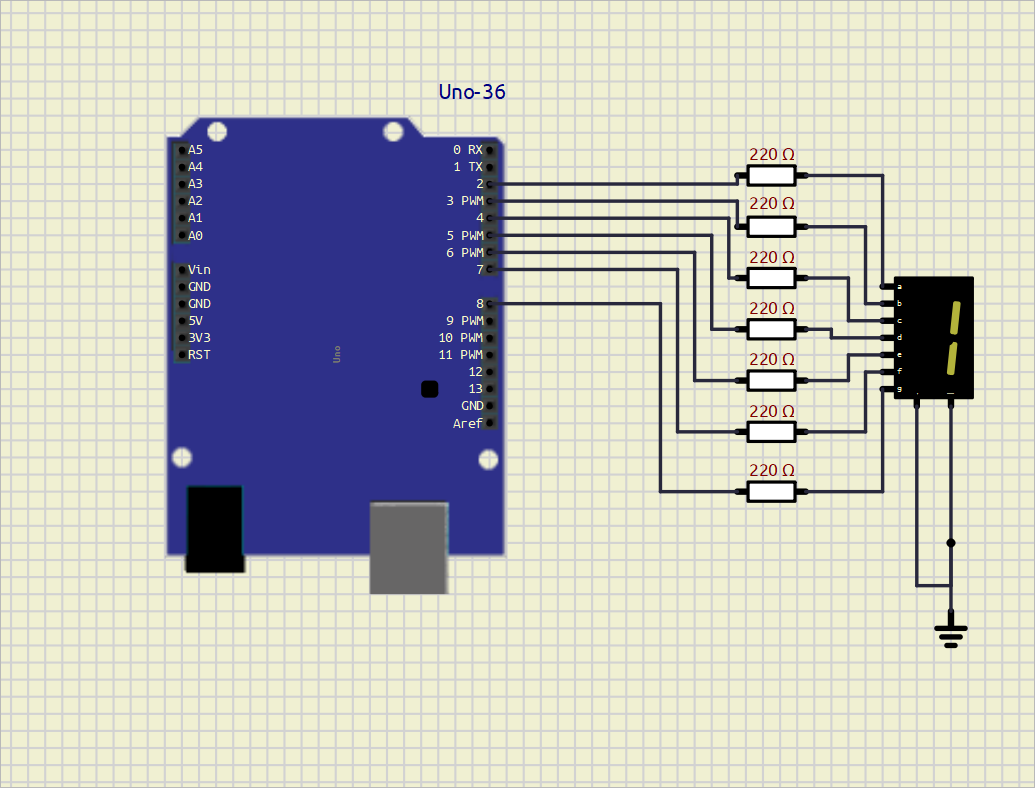
\includegraphics[width=\linewidth]{Exp-0/7_segment_led/7_Segment_Led.png}
\end{minipage}
\hfill
\begin{minipage}{0.48\textwidth}
    \centering
    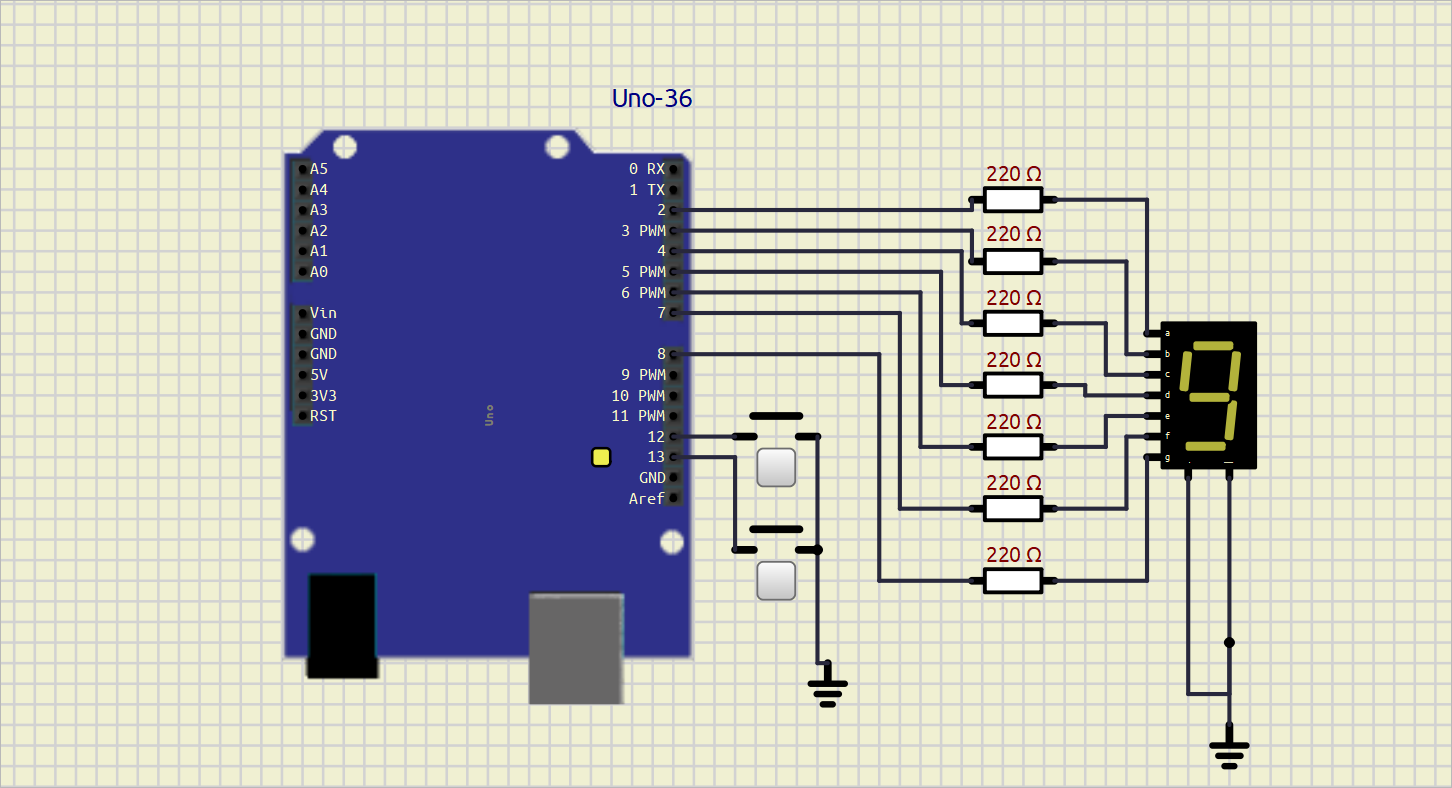
\includegraphics[width=\linewidth]{Exp-0/7_segment_led/7-Segment with push botton.png}
\end{minipage}

\caption{Circuit Diagram of 7-Segment Display Interfacing}
\label{fig:7segment}
\end{figure}

%%%%%%%%%%%%%%%%%%%%%%%%%%%%%%%%%%%%%%%%%%%%%%%%%%%%%%%%%%%%%%%%%%%%%%%

\subsection{Source Code}

The complete Arduino source code for this experiment is available in the project repository.

\href{https://github.com/YOUR_USERNAME/YOUR_REPOSITORY/blob/main/Exp-0/7_segment_led/file.ino}
{\textbf{Click here to view the Arduino Source Code}}

%%%%%%%%%%%%%%%%%%%%%%%%%%%%%%%%%%%%%%%%%%%%%%%%%%%%%%%%%%%%%%%%%%%%%%%

\subsection{Working Principle}

\begin{enumerate}

\item The 7-segment display segments are connected to Arduino digital pins D2 to D8.

\item Each segment is controlled individually using \texttt{digitalWrite()}.

\item Depending on which segments are turned ON or OFF, different numbers are displayed.

\item The Arduino sequentially displays:

\begin{itemize}
\item 0 \item 1 \item 2 \item 3
\end{itemize}

\item Each number remains visible for 1 second using \texttt{delay(1000)}.

\item The sequence repeats continuously.

\end{enumerate}

%%%%%%%%%%%%%%%%%%%%%%%%%%%%%%%%%%%%%%%%%%%%%%%%%%%%%%%%%%%%%%%%%%%%%%%

\subsection{Learning Outcomes}

\begin{itemize}

\item Interfacing a 7-segment display with Arduino UNO

\item Common cathode display working principle

\item Using multiple digital output pins

\item Number display logic using segments

\item Arduino digital output voltage is approximately 5V

\item Recommended current per pin is 20mA

\item Typical LED segment current is around 10mA to 20mA

\end{itemize}

%%%%%%%%%%%%%%%%%%%%%%%%%%%%%%%%%%%%%%%%%%%%%%%%%%%%%%%%%%%%%%%%%%%%%%%

\subsection{Conclusion}

The 7-segment display was successfully interfaced with Arduino UNO.

The display sequentially showed numbers from 0 to 3 by controlling individual segments through Arduino digital pins. This project helped in understanding display interfacing and segment control logic.

%%%%%%%%%%%%%%%%%%%%%%%%%%%%%%%%%%%%%%%%%%%%%%%%%%%%%%%%%%%%%%%%%%%%%%%

\subsection{References}

\begin{enumerate}

\item Arduino Official Website

\url{https://www.arduino.cc/}

\item Arduino UNO Documentation

\url{https://docs.arduino.cc/hardware/uno-rev3/}

\item 7-Segment Display Basics

\url{https://www.electronics-tutorials.ws/blog/7-segment-display-tutorial.html}

\item Arduino Tutorials

\url{https://www.arduino.cc/en/Tutorial/HomePage}
\end{enumerate}

%%%%%%%%%%%%%%%%%%%%%%%%%%%%%%%%%%%%%%%%%%%%%%%%%%%%%%%%%%%%%%%%%%%%%%%

\clearpage
Experiment 0 (Go Further 2)

\section{LED Matrix Emoji Display System}


%%%%%%%%%%%%%%%%%%%%%%%%%%%%%%%%%%%%%%%%%%%%%%%%%%%%%%%%%%%%%%%%%%%%%%%

\subsection{Problem Statement}

The objective of this project is to interface an 8×8 LED matrix with Arduino UNO and display different emoji patterns.

This experiment helps in understanding:

\begin{itemize}
    \item LED matrix interfacing
    \item Row and column scanning
    \item Pattern generation
    \item Multiplexing technique
\end{itemize}

%%%%%%%%%%%%%%%%%%%%%%%%%%%%%%%%%%%%%%%%%%%%%%%%%%%%%%%%%%%%%%%%%%%%%%%
\subsection{Components Used \& Pin Connections}

\begin{table}[H]
\centering
\caption{LED matrix Components Used and Pin Connections}
\label{tab:ledmatrix}

\begin{tabular}{|l|c|l|c|}
\hline
\multicolumn{2}{|c|}{\textbf{Components}} &
\multicolumn{2}{c|}{\textbf{Pin Connections}}\\
\hline
Arduino UNO & 1 & Row 1 & D1\\
8×8 LED Matrix & 1 & Row 2 & D2\\
125$\Omega$ Resistors & 8 & Row 3 & D3\\
Breadboard & 1 & Row 4 & D4\\
Jumper Wires & Required & Row 5 & D5\\
 &  & Row 6 & D6\\
 &  & Row 7 & D7\\
 &  & Row 8 & D8\\
 &  & Column 1 & A5\\
 &  & Column 2 & A4\\
 &  & Column 3 & A3\\
 &  & Column 4 & A2\\
 &  & Column 5 & D9\\
 &  & Column 6 & D10\\
 &  & Column 7 & D11\\
 &  & Column 8 & D12\\
\hline
\end{tabular}

\end{table}
%%%%%%%%%%%%%%%%%%%%%%%%%%%%%%%%%%%%%%%%%%%%%%%%%%%%%%%%%%%%%%%%%%%%%%%

\subsection{Software Used}

\begin{itemize}
    \item Arduino IDE
    \item Proteus / SimulIDE
\end{itemize}

%%%%%%%%%%%%%%%%%%%%%%%%%%%%%%%%%%%%%%%%%%%%%%%%%%%%%%%%%%%%%%%%%%%%%%%

\subsection{Circuit Diagram}

\begin{figure}[H]
\centering

\includegraphics[width=0.6\textwidth]{Exp-0/Led_Matrix_8X8/Led_ Matrix_ Circuit.png}
\caption{Circuit Diagram of LED Matrix Emoji Display System}
\label{fig:ledmatrix}
\end{figure}

%%%%%%%%%%%%%%%%%%%%%%%%%%%%%%%%%%%%%%%%%%%%%%%%%%%%%%%%%%%%%%%%%%%%%%%

\subsection{Source Code}

The complete Arduino source code for this experiment is available in the project repository.

\href{https://github.com/YOUR_USERNAME/YOUR_REPOSITORY/blob/main/Exp-0/Led_Matrix_8X8/file.ino}
{\textbf{Click here to view the Arduino Source Code}}

%%%%%%%%%%%%%%%%%%%%%%%%%%%%%%%%%%%%%%%%%%%%%%%%%%%%%%%%%%%%%%%%%%%%%%%

\subsection{Working Principle}

\begin{enumerate}

\item The 8×8 LED matrix is connected to Arduino UNO using row and column connections.

\item Arduino scans rows and columns rapidly using multiplexing.

\item Binary patterns are stored inside the \texttt{emoji} array.

\item The \texttt{displayEmoji()} function activates rows one by one and controls columns according to the stored pattern.

\item Different emoji patterns are displayed continuously on the LED matrix.

\item Due to fast scanning, the complete image appears continuously visible.

\end{enumerate}

%%%%%%%%%%%%%%%%%%%%%%%%%%%%%%%%%%%%%%%%%%%%%%%%%%%%%%%%%%%%%%%%%%%%%%%

\subsection{Learning Outcomes}

\begin{itemize}

\item Interfacing an LED matrix with Arduino UNO

\item Multiplexing technique

\item Row and column scanning

\item Pattern generation using binary values

\item Arduino digital output voltage is approximately 5V

\item Recommended current per pin is 20mA

\item LED matrix LEDs require current limiting resistors

\end{itemize}

%%%%%%%%%%%%%%%%%%%%%%%%%%%%%%%%%%%%%%%%%%%%%%%%%%%%%%%%%%%%%%%%%%%%%%%

\subsection{Conclusion}

The LED matrix was successfully interfaced with Arduino UNO.

Different emoji patterns were displayed by controlling rows and columns using multiplexing techniques. This project helped in understanding matrix displays and pattern generation in embedded systems.

%%%%%%%%%%%%%%%%%%%%%%%%%%%%%%%%%%%%%%%%%%%%%%%%%%%%%%%%%%%%%%%%%%%%%%%

\subsection{References}

\begin{enumerate}

\item Arduino Official Website

\url{https://www.arduino.cc/}

\item Arduino UNO Documentation

\url{https://docs.arduino.cc/hardware/uno-rev3/}

\item LED Matrix Basics

\url{https://www.electronicsforu.com/resources/learn-electronics/8x8-led-matrix-module}

\item Arduino Tutorials

\url{https://www.arduino.cc/en/Tutorial/HomePage}

\end{enumerate}